\documentclass{article}

\usepackage{fontspec}
\usepackage{polyglossia}
\usepackage{graphicx}
\usepackage{csquotes}

\setdefaultlanguage{french}
\MakeOuterQuote{"}

\title{Compte-rendu \\ \smallskip \large du projet de Web de S2}
\author{Jean Evrat \and Elouan Fabre \and Quentin Laget \and Ali El Mahouli}

\begin{document}

\maketitle

\section*{Introduction}

Notre projet pour l'enseignement de programmation Web pouvait prendre différente formes. Des sujets nous étaient proposés. En particulier, il nous était possible de choisir un sujet personnalisé, de faire notre propre site Internet sur un thème de notre choix. Après examen des sujets proposés nous est venu une idée pour le sujet libre: celle de créer une plateforme de dépôt de sujets d'oraux à destination des élèves de classe préparatoire. Ce sujet nous séduisit et fut adopté après l'approbation de notre professeur référent.

Bien que, nous en étions conscients, le site que nous allions créer s'inscrivait dans un cadre scolaire, nous n'avons pas tardé à imaginer concrètement ce que pourrait devenir le site s'il était mis en ligne avec une réelle intention de rendre service à des élèves. En effet, il nous est apparu que ce genre de site manquait en ligne, ou bien étaient difficilement accessibles (sites lourds, dont l'administration peut interroger, au contenu quelquefois payant, avec des publicités, ou bien avec du contenu périmé). Notre volonté de créer ce site ne partait donc pas seulement de l'école, mais aussi d'une intiative de créer quelque chose d'inexistant, d'utile, de libre et d'accessible, pour éventuellement le partager en ligne.

S'ensuivit alors des questions très pratiques que nous nous sommes soulevées. Comment permettre au plus de personnes possible de proposer un sujet, mais qu’il soit à la fois de qualité? Comment permettre un accès rapide à l'information sans que l'utilisateur se perde dans le nombre et une interface compliquée?


\section*{Mise en place du projet et répartition des rôles}

Nous avons commencé relativement tôt à travailler sur le site dont le développement nous motivait, en parallèle des autres projets. Nous avons utilisé un dépôt git hébergé sur \texttt{gitlab.pedago.ensiie.fr}, sur lequel nous avons travaillé en privé entre membres de notre groupe sobrement intitulé "Les Moutons du Purgatoire". Nous avons séparé notre travail en plusieurs parties: le dépôt de documents, la consultation de documents, la gestion de la connexion et de la création d'un utilisateur, la gestion des profils d'un utilisateur, ainsi que l'interface. Après consultation, il fut convenu que Ali El Mahouli s'occuperait de la recherche d'un sujet, de la consultation d'un profil, de la rédaction des commentaires, que Jean Evrat s'occuperait de la connexion d'un utilisateur et de la modification d'un profil, que Elouan Fabre s'occuperait du dépôt d'un document, et qu'enfin Quentin Laget s'occuperait de l'interface gérée par CSS. Finalement, en fonction de l'avancement de chacun dans le projet, des dépendances des pages entres elles et des moments de grande motivation de la part de certains, il arrivait que nous nous attribuions d'autres tâches, l'essentiel étant que le projet avançât. Cette organisation nous permit de finir le site de la manière dont nous le souhaitions.


\section*{Développement}

\subsection*{Jean Evrat}

La première difficulté rencontrée au cours de ce projet était tout simplement la nouveauté du langage. Nous sommes ainsi partis sur des solutions qui n'étaient pas forcément les meilleures et qui impliquaient de recommencer le travail à 0 si nous souhaitions les modifier. Par exemple, le non-usage de fonctions ou de classes comme celles données en exemple dans le sujet de départ auraient pu être judicieuses mais nous n'y avons pas pensé immédiatement.

Nous avancions en choisissant au fur et à mesure les fonctionnalités que nous souhaitions faire individuellement, à partir de la base d'idées définies au départ. J'ai débuté par la connexion à la base de données (création et instauration de mot de passe) en collaboration avec Ali El Mahouli.  Afin d'uniformiser la bdd chez tout le monde et travailler sur une même base, nous avons pris la décision de maintenir un fichier \texttt{.sql} qui la définirait et que l'on mettrait à jour à chaque changement.

Mon travail suivant fut l'enregistrement d'un membre. Il suffisait de demander à la personne souhaitant s'inscrire ses identifiants et de les enregistrer dans la bdd. Cependant, au fur et à mesures des modifications apportées au projet et des nouvelles idées (récupération d'un mot de passe...), les deux fichiers correspondants. Cela ne fut pas très difficile dans l'ensemble pusique le code nécessaire était initialement assez simple, mais il a fallu y revenir tout au long du projet, rendant le code de plus en plus complexe.

Ensuite, je me chargeai de la récupération du mot de passe, demandée par un utilisateur existant, à l'aide d'une question. J'eu beaucoup de mal avec cette fonctionnalité. En effet, cela demandait un mélange de PHP et HTML dans certains fichiers alors que j'essayais de séparer les fichiers entre ceux en HTML et ceux en PHP. En outre, il m'a fallu faire un postage (avec \texttt{<form>}) automatique, chose que j'ai réussie après de nombreux essais grâce à une fonction en javascript.

À nouveau, l'inexpérience dans le domaine du langage Web m'a posé problème pusique je n'arrivais pas à me débrouiller avec les nombreuses variables à traiter. C'est en partie pour cela qu'il y a 4 fichiers correspondant à la récupération du mot-de passe, chose qui alourdit inutilement le travail alors qu'il aurait été facile d'utiliser des variables globales ou la classe proposée au départ.

J'ai ensuite essayé de demander un mail pour avoir une validation d'inscription classique. Cependant, la fonction mail de php était bloquée sur les boites mails classiques car considérée comme pire qu'un spam, et je n'arrivais pas à utiliser PHPmailer. J'ai donc confié cette tâche à mon camarade Ali El Mahouli.

La fonctionnalité suivante fut le dépot d'une photo de profil lors de l'enregistrement. J'ai eu quelques soucis, le premier étant l'oubli de la précision du dépot de fichier dans le \texttt{<form>}. Ceci m'a fait tourner en rond pendant un petit bout de temps.

En second lieu, ce fut la mise à jour de cette photo qui me posa problème: il fallait pouvoir la retouver facilement, j'ai donc pris la décision de la renommer en fonction du nom de l'utilisateur en supprimant celle déjà existante. Ainsi, on facilite le repérage dans la bdd et dans le fichier des photos.

Enfin, je fus chargé de l'arborescence du projet car tous nos fichiers étaient dans le même répertoire. Il a donc fallu parcourir chaque fichier pour pouvoir les remettre dans une configuration correcte, notamment lors des appels inter-fichiers. Ce n'était pas particulièrement difficile mais un peu fastidieux et il fallait une bonne compréhension du code pour pouvoir retrouver tous les appels de fichiers pour les mettre à jour.


\subsection*{Elouan Fabre}

Ce projet de programmation Web était pour moi une opportunité de mettre en pratique les enseignements de l'école et ma créativité. J'ai eu l'idée du thème que nous avons choisi avant même d'avoir lu le sujet du projet de programmation Web. Quand j'étais en classe préparatoire, un des professeur de l'équipe pédagogique a eu l'idée de lancer un site en ligne sur lequel tous les élèves pourraient y partager les planches d'oral qu'ils avaient eues lors de leurs oraux, afin d'en faire profiter tout le monde. Le problème, c'est que son site était inutilement lourd, mal présenté, et était couvert de publicités (quelquefois louches d'ailleurs) pour payer les frais d'hébergements. C'est lorsque j'ai vu cela que l'idée d'un site du même acabit, mais plus simple, sans publicité et éventellement sous license libre en cas de partage, m'est apparue.

Le site s'est concrétisé avec l'aide de mes camarades. J'ai particulièrement participé aux réflexions sur l'interface, sur les possibilités que pouvaient avoir un utilisateur lambda, et sur les questions de maintenance; fallait-il autoriser n'importe quel état de rendu d'un sujet d'oral, car les candidats ne peuvent pas conserver le sujet qui leur est donné à l'oral, et n'ont quelquefois que des brouillons à partager? Un utilisateur a-t-il besoin d'être inscrit pour ajouter un sujet? Faut-il ajouter un système de notation sur les sujets?

Toutes ces questions m'ont amené à me poser la question du respect du droit d'auteur dans notre site; de nombreux corrigés de sujets écrits ou oraux sont souvent proposés sur Internet, mais bien souvent sous license protégée, ou ambigüe (dans l'Union européenne, un travail de ce genre est placé par défaut sous une license très restrictive dont il est possible de s'échaper seulement en cas d'autorisation explicite de l'auteur). De plus, si un étudiant se rappelle exactement un sujet, a-t-il le droit de le poster mot pour mot tel que l'on lui a présenté sur un site?

Après ces questions fondamentales que je me suis posées et la contribution à l'énonciation des lignes directrices, d'idées pour l'interface, venait le temps de la pratique. Je me suis très vite heurté à quelques problèmes avec PostgreSQL sur mon ordinateur que mes camarades n’avaient pas; en effet, à chaque tentative de connection à la base de donnée avec l'utilisateur \texttt{postgres} par défaut, je me heurtais à l'erreur suivante: \texttt{psql: FATAL:  authentification Ident échouée pour l'utilisateur « postgres »}, ce qui m'a freiné dans mon développement. Après de nombreuses recherches, j'ai réussi à me débarrasser de cette erreur avec la modification du fichier de configuration des accès réseaux à la base de donnée, \texttt{/var/lib/pgsql/data/pg\_hba.conf} dans lequel j'ai dû mettre la méthode sur \texttt{TRUST} pour tous les types de connection, sauf pour l'IPv6. Cette erreur réglée, j'ai pu contribuer au projet.

Étant assez pointilleux, j'ai contribué au projet tout d'abord en veillant à l'orthographe, à la typographie (espace fine insécables devant les points d'exclamation et d'interrogation, etc.), à la lisibilité ainsi qu'à la gestion de la mise en page, de l'emplacement des boutons, ainsi qu'à l'interface globale du site, pour permettre plus de fluidité à l'expérience de l'utilisateur. J'ai aussi veillé à la lisibilité du code source. Ma contribution a été aussi d'aider au débogage de problèmes liés à la base de données avec Ali El Mahouli.


\subsection*{Quentin Laget}

Après la mise en place des bases de données par mes camarades, un problème de taille s'est vite imposé à moi. Ayant pour habitude de travailler sous Windows avec un terminal en bash, je devais installer les extensions permettant de manipuler les bases de données dans mon terminal. Étant donné qu'il est impossible d'utiliser les fonctions liées à sudo dans Windows, j'ai essayé d'avoir recours à d'autres méthodes pour accéder aux fonctions de PgSQL.

J'ai d'abord installé un package php-pgsql dans le terminal que j'utilise (MobaXterm). L'utilisation des fonctions de PgSQL s'est néanmoins révélée impossible: en effet, toute fonction liée aux bases de données ne s'arrêtait pas: il m'est alors impossible d'accéder ou de modifier les bases de données.  Après plusieurs recherches, il s'est avéré qu'il y avait un conflit avec les droits administrateurs de Windows qui m'empêchaient d'accéder aux bases de données. Malgré les changements des droits administrateurs, le problème persiste.

J'ai alors essayé de télécharger les fonctions de PgSQL non plus dans le terminal, mais dans mes variables d'environnement système. Malheureusement, rien n'a changé. J'ai alors tenté d'avoir recours à une machine virtuelle pour faire tourner ces fonctions, sans succès. D'un commun accord avec le reste du groupe, il a été décidé que je m'occuperai de la mise en forme du site avec notamment les fichiers PHP et les feuilles de style CSS, qui ne nécessitent pas un accès aux bases de données.

Après la réalisation des maquettes du site par les autres membres du groupe, une autre difficulté qui s'est imposée est l'impossibilité de visualiser les pages du site. En dehors du terminal, j'ai alors décidé d'installer le logiciel Xampp, qui permet de visualiser des pages PHP avec leurs feuilles de style sous Windows. Une fois le logiciel installé, j'ai enfin pu accéder au rendu des différentes pages PHP en déplaçant tous les fichiers dans un dossier spécifique à Xampp.

La prise en main des langages CSS et PHP a été assez rapide et j'ai vite pu m'atteler à la tache qui m'incombe. Après concertations avec les autres membres du groupe et plusieurs propositions de style, j'ai préféré adopté un style unique pour toutes les pages qui reste sobre mais fonctionnel.


\subsection*{Ali El Mahouli}

Pour commencer, il nous fallait une page de connexion. J'ai donc créé une première table dans la base de données avec un nom d'utilisateur comme clé primaire et un mot de passe. Cette table sera ensuite modifiée pour ajouter plus d'informations sur l'utilisateur, Jean Evrat en avait besoin notamment pour la création de compte et la récupération du mot de passe.

J'ai ensuite modifié le \texttt{index.html} pour afficher un formulaire qui demande le nom d'utilisateur et le mot de passe. J'ai créé \texttt{login.php} pour gérer la connexion, elle établit la connexion à la base de données et recherche l'utilisateur. Si le visiteur du site veut créer un compte ou a oublié son mot de passe il pourra cliquer sur les liens des pages de création de compte ou de récupération de mot de passe créés par mon camarade Jean Évrat.

Le visiteur peut toutefois accéder au site en cliquant sur \texttt{Accueil} dans le header. Cependant, il n'aura pas droit à toutes le fonctionnalités : notamment le dépôt de sujet, la possibilité de commenter ou de proposer une correction d'un sujet existant.

Une fois l'utilisateur connecté, il se trouve sur une page \texttt{accueil.php} qui lui donne le choix entre déposer un sujet ou en consulter un.

Si l'utilisateur choisit de chercher un sujet il est tranféré à la page \texttt{recherche.php} qui est un formulaire de recherche basé sur la matière du sujet, l'année, le concours, la filière et le thème. Les thèmes changent en fonction de la matière choisie à l'aide d'un code JavaScript. Cette partie m'avait pris assez de temps, d'un côté parce que ce formulaire de recherche était la fonctionnalité essentielle du site mais aussi le fait de changer les options des thèmes était pour nous nécessaire, pour avoir un formulaire plus logique.

Une fois les informations validées, la page \texttt{find.php} se charge de se connecter à la base de données et de retrouver les sujets qui vérifient les conditions. Elle rassemble les identifiants des sujets concernés dans un \texttt{array} qu'elle transmet à \texttt{resultat.php}.
La table qui gère les sujets dans la base de données contient comme attributs: l'identifient du sujet, le nom du fichier, l'utilisateur qui l'a publié, le concours dans lequel il s'inscrit, la filière, la matière, l'année et le thème.

La page \texttt{resultat.php} affiche une liste des liens vers des pages qui décrivent les sujets possibles. C'est la page \texttt{sujet.php}.

La page \texttt{sujet.php} permet de gérer les fonctionnalités liées à un sujet donné: Consulter le sujet, proposer une correction, consulter les corrections, commenter, répondre à un commentaire. Si le sujet a été publié par l'utilisateur, ou s'il est administrateur, il pourra le supprimer. Si l'utilisateur souhaite proposer une correction il sera redirigé vers la page \texttt{correction.php} où il pourra choisir le fichier de correction, qui sera rajouté par \texttt{uploadcorrection.php} s'il vérifie certaines conditions de taille et de type.

\textbf{Les commentaires:} pour gérer les commentaires, j'ai créé la table \texttt{comment} qui a comme attributs: l'identifiant du sujet, l'identifiant du commentaire, le contenu du commentaire et l'identifiant du commentaire auquel il répond s'il s'agit d'une réponse.

\textbf{Les corrections:} pour gérer les corrections, j'ai créé la table \texttt{correction} qui a comme attributs: l'identifiant du sujet auquel elle correspond, le nom du fichier et le nom d'utilisateur qui l'a publiée.

On envoie un mail à l'utilisateur si un nouveau commentaire est rajouté à sa publication. Il est informé du nom de la publication dans le mail. Ceci est effectué par \texttt{mailcomment.php} (figure \ref{mail}).

\begin{figure}[h]
\centering
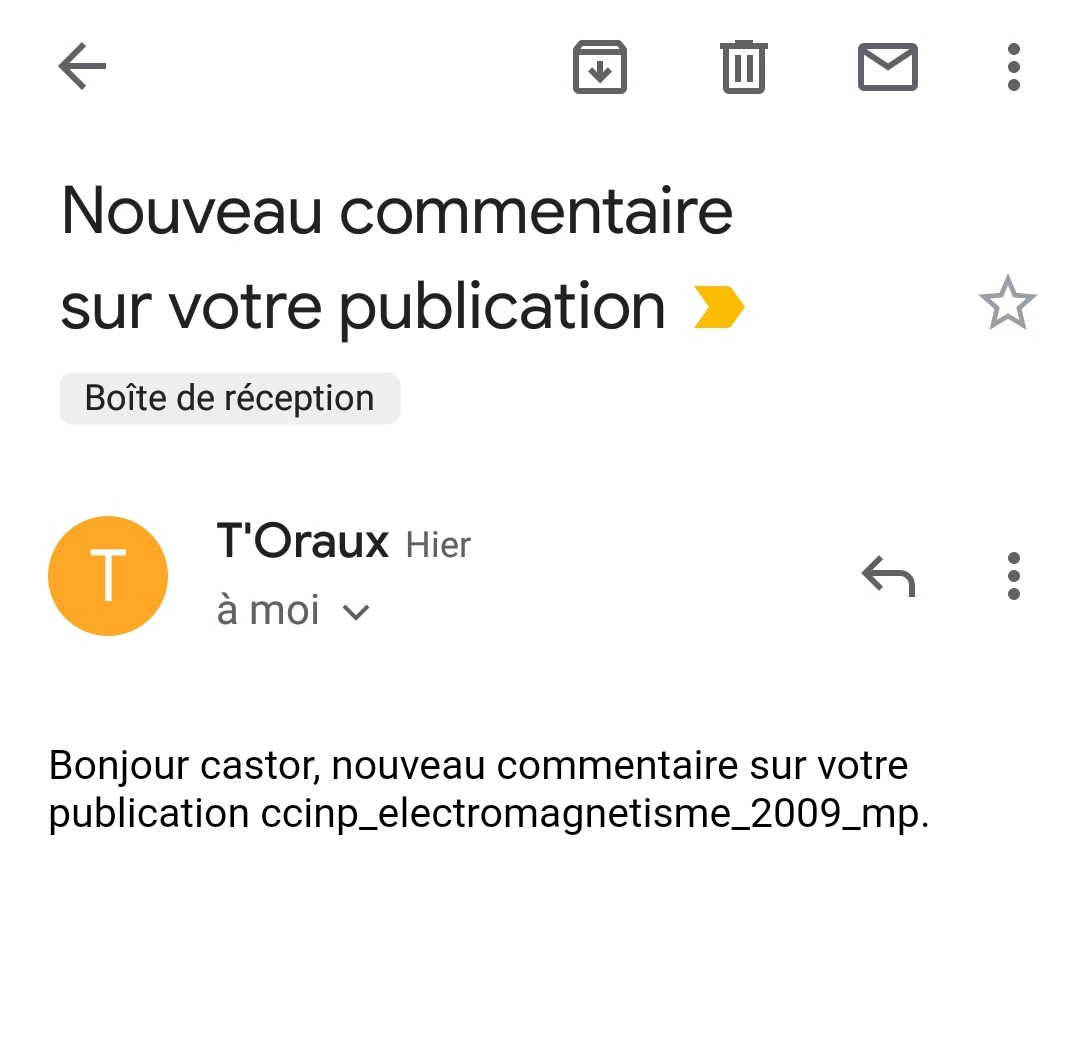
\includegraphics[width=8cm]{mail.jpg}
\caption{Mail reçu par l'utilisateur si un nouveau commentaire est ajouté à sa publication.}
\label{mail}
\end{figure}

Si l'utilisateur choisit de déposer un document. Il sera transféré à la page \texttt{depot.php} où il pourra entrer des details sur le sujet qu'il dépose. Le formulaire a les mêmes composants que le formulaire de recherche, cependant un sujet correspond à un seul concours et une seule filière et un seul thème, il n'aura pas de choix multiple pour ces éléments.

\texttt{uploadsujet.php}: traite le formulaire de dépôt. On teste d'abord si l'utilisateur est connecté, si non on l'informe qu'il doit se connecter pour déposer un fichier. On vérifie le type du fichier importé, sa taille. S'ils conviennent, on teste si la matière a bien été indiquée. Si oui, on initie la commande d'insertion avec les champs dont on dispose nécessairement. Ensuite on parcourt les autres champs, on insère leur valeur si elle est mentionnée.

Si l'utilisateur clique sur le lien \texttt{Mon Profil} dans le \texttt{header} ou s'il clique sur le nom d'un utilisateur dans une section de commentaires, il sera transféré à la page \texttt{profil.php} où il pourra retrouver des informations sur l'utilisateur. Si l'utilisateur possède le compte en question il pourra modifier ses informations, il sera redirigé vers une page créée par mon camarade Jean Evrat. Il pourra aussi supprimer son compte. S'il est administrateur il pourra supprimer le compte de tout utilisateur.

Si l'utilisateur (connecté ou pas) clique sur le lien \texttt{Contact} dans le \texttt{header}, il sera transféré à la page \texttt{contact.php} ou il pourra retrouver un formulaire qui lui permet de contacter les administrateurs. Il doit mentionner son nom, son adresse mail et son message. Les informations sont ensuite transférées à \texttt{sendcontact.php} qui envoie un mail à des adresses d'administrateurs précises avec le contenu du formulaire (figure \ref{commentaire}).

\begin{figure}[h]
\centering
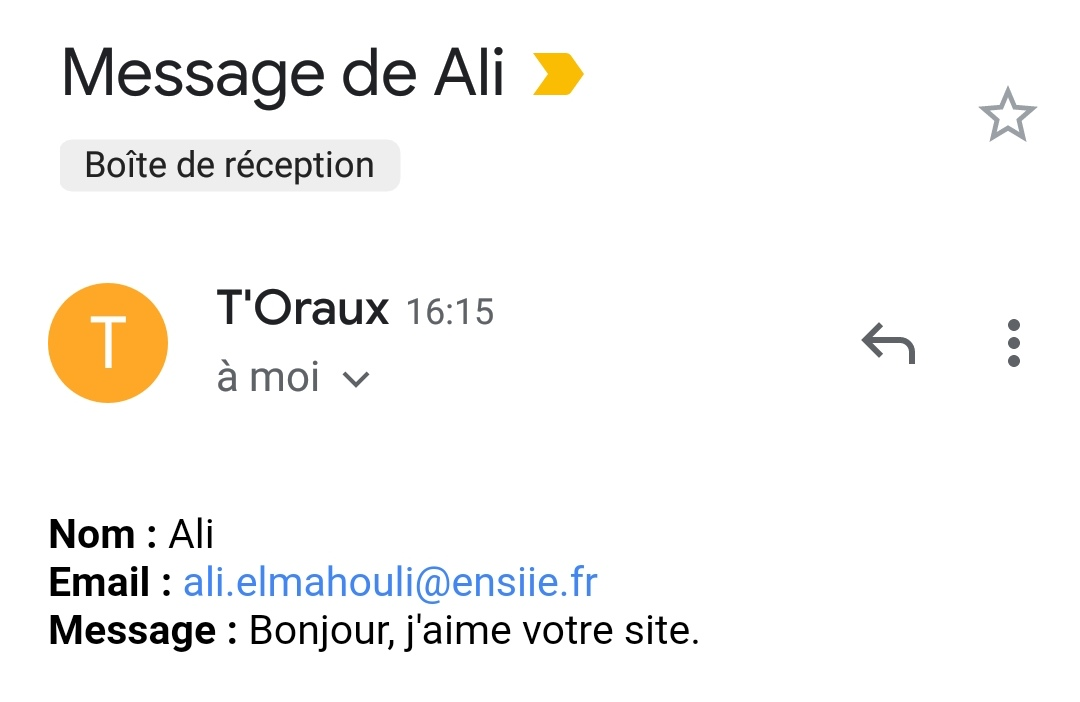
\includegraphics[width=8cm]{commentaire.jpg}
\caption{Mail reçu par les administrateurs.}
\label{commentaire}
\end{figure}

Pour la mise en page, j'ai travaillé avec mon camarade Quentin Laget pour choisir un logo, des couleurs d'arrière-plan et de boutons. Finalement on a choisi quelque chose de simple. J'ai également fait la mise en page des différents boutons des pages et du header. La plupart des pages ont une feuille de CSS \texttt{style2.css} sauf si la page nécessite quelques changements.

Les difficultés que j'ai rencontrées sont celles liées à la manipulation d'un langage avec lequel je n'ai pas eu beaucoup d'expérience. Aussi, le fait de séparer les fonctionnalités entre celle accessbles à tout le monde d'autres aux utilisateur connectés et d'autres aux administrateur. J'ai eu donc multiplier les tests. L'utilisation de PHPMailer a été difficile aussi, j'ai du essayer différents paramètres pour réussir à envoyer les mails. J'ai pensé à héberger le site sur un domaine gratuit, mais la plupart des sites gratuits que j'ai trouvé utilisait Mysql pour la gestion des bases de données.


\section*{Bilan}

Ce projet nous a beaucoup apporté, autant dans l'organisation du travail en groupe que dans la maîtrise du langage de développement Web, qui nous était presque inconnu. Nous avons appris à composer avec nos différents problèmes et à trouver des arrangements qui permettait à chacun de trouver son rôle.

\end{document}
